\subsection{Execution Flow}
\label{flow}

Now that we know the different plugin types and their operation that are involved in the bootstrapping process, we can present a step-by-step description of the whole process.
\autoref{image:flow} shows a graph that represents the major steps during the bootware execution as flow diagram.
What follows is the description of the whole process.

The bootstrapping process is started by executing the bootware, which is represented by the start state in the top left corner of \autoref{image:flow}.
From there, the bootware first does some initializations.
If these fail for some reason, the cleanup code will be executed before the bootware execution is ended, as can be seen on the top right corner of \autoref{image:flow}.
In most cases however, the initialization should succeed.
Then, the bootware will transition to the next state, where it tries to load the event plugins.

The event plugins are loaded once at the beginning of the bootware execution, since they will not change at a per request basis (like the other plugins).
If loading these plugins fails, the bootware will try to unload them before continuing to the cleanup state.
If the plugins are loaded successfully, the bootware transitions into the wait state, shown in the top center of \autoref{image:flow}.

Once the bootware is in the wait state it is ready to receive requests from the outside.
If a shutdown event is received in this state, the bootware will start the shutdown procedure by first unloading the event plugins and then running the cleanup code.
This is the only normal way to shutdown the bootware.
If a request is received in the wait state, the bootware transitions to the next state, where it reads the request context.

The request context contains all the information necessary to fulfill the request.
This includes, among others, the type of the request(deploy or undeploy), the login credentials for a cloud provider, and the names of one of each of the infrastructure, connection, and payload plugin to be used during the bootstraping process.
If the context can not be read, the bootware returns a response containing an error message before returning into the wait state.
If the context is read successfully the bootware transitions to the load request plugins state.

In the load request plugins state the three plugins specified in the context are loaded.
If this fails, the bootware tries to unload them before return an error response and returning to the wait state.
If the plugins are loaded successfully, the bootware now starts either the deploy process or the undeploy process, shown at the bottom of \autoref{image:flow}, depending on the type of the request.

If the request was a deploy request, the bootware will now execute the deploy, connect, and start operations of the infrastructure, connection, and payload plugins, one after another.
If one of those operations fails the bootware transitions over to the corresponding undeploy operation and works its way backwards to undo all operations that where already executed.
This process is the same as the undeploy process trigger by an undeploy request.

If the stop payload, deprovision payload, or disconnect states fail, the bootware just continues with the next undeploy state, since these operations are not considered critical.
However, if the deprovision infrastructure state fails, the bootware transitions to a fatal error state, show at the right of \autoref{image:flow}, since this step is considered critical.
This state failing could mean that resources are still active in the cloud and human interaction is necessary to remove them to stop further costs from incurring.
The fatal error state is responsible for informing the user that he has to interfere.

The successful, as well as the unsuccessful execution of either the deploy or the undeploy process all finish in the unload request plugin state, where the plugins that where needed for this particular request are unloaded, before a suitable response is returned and the bootware returns to the wait state.

\begin{figure}[!htbp]
	\centering
	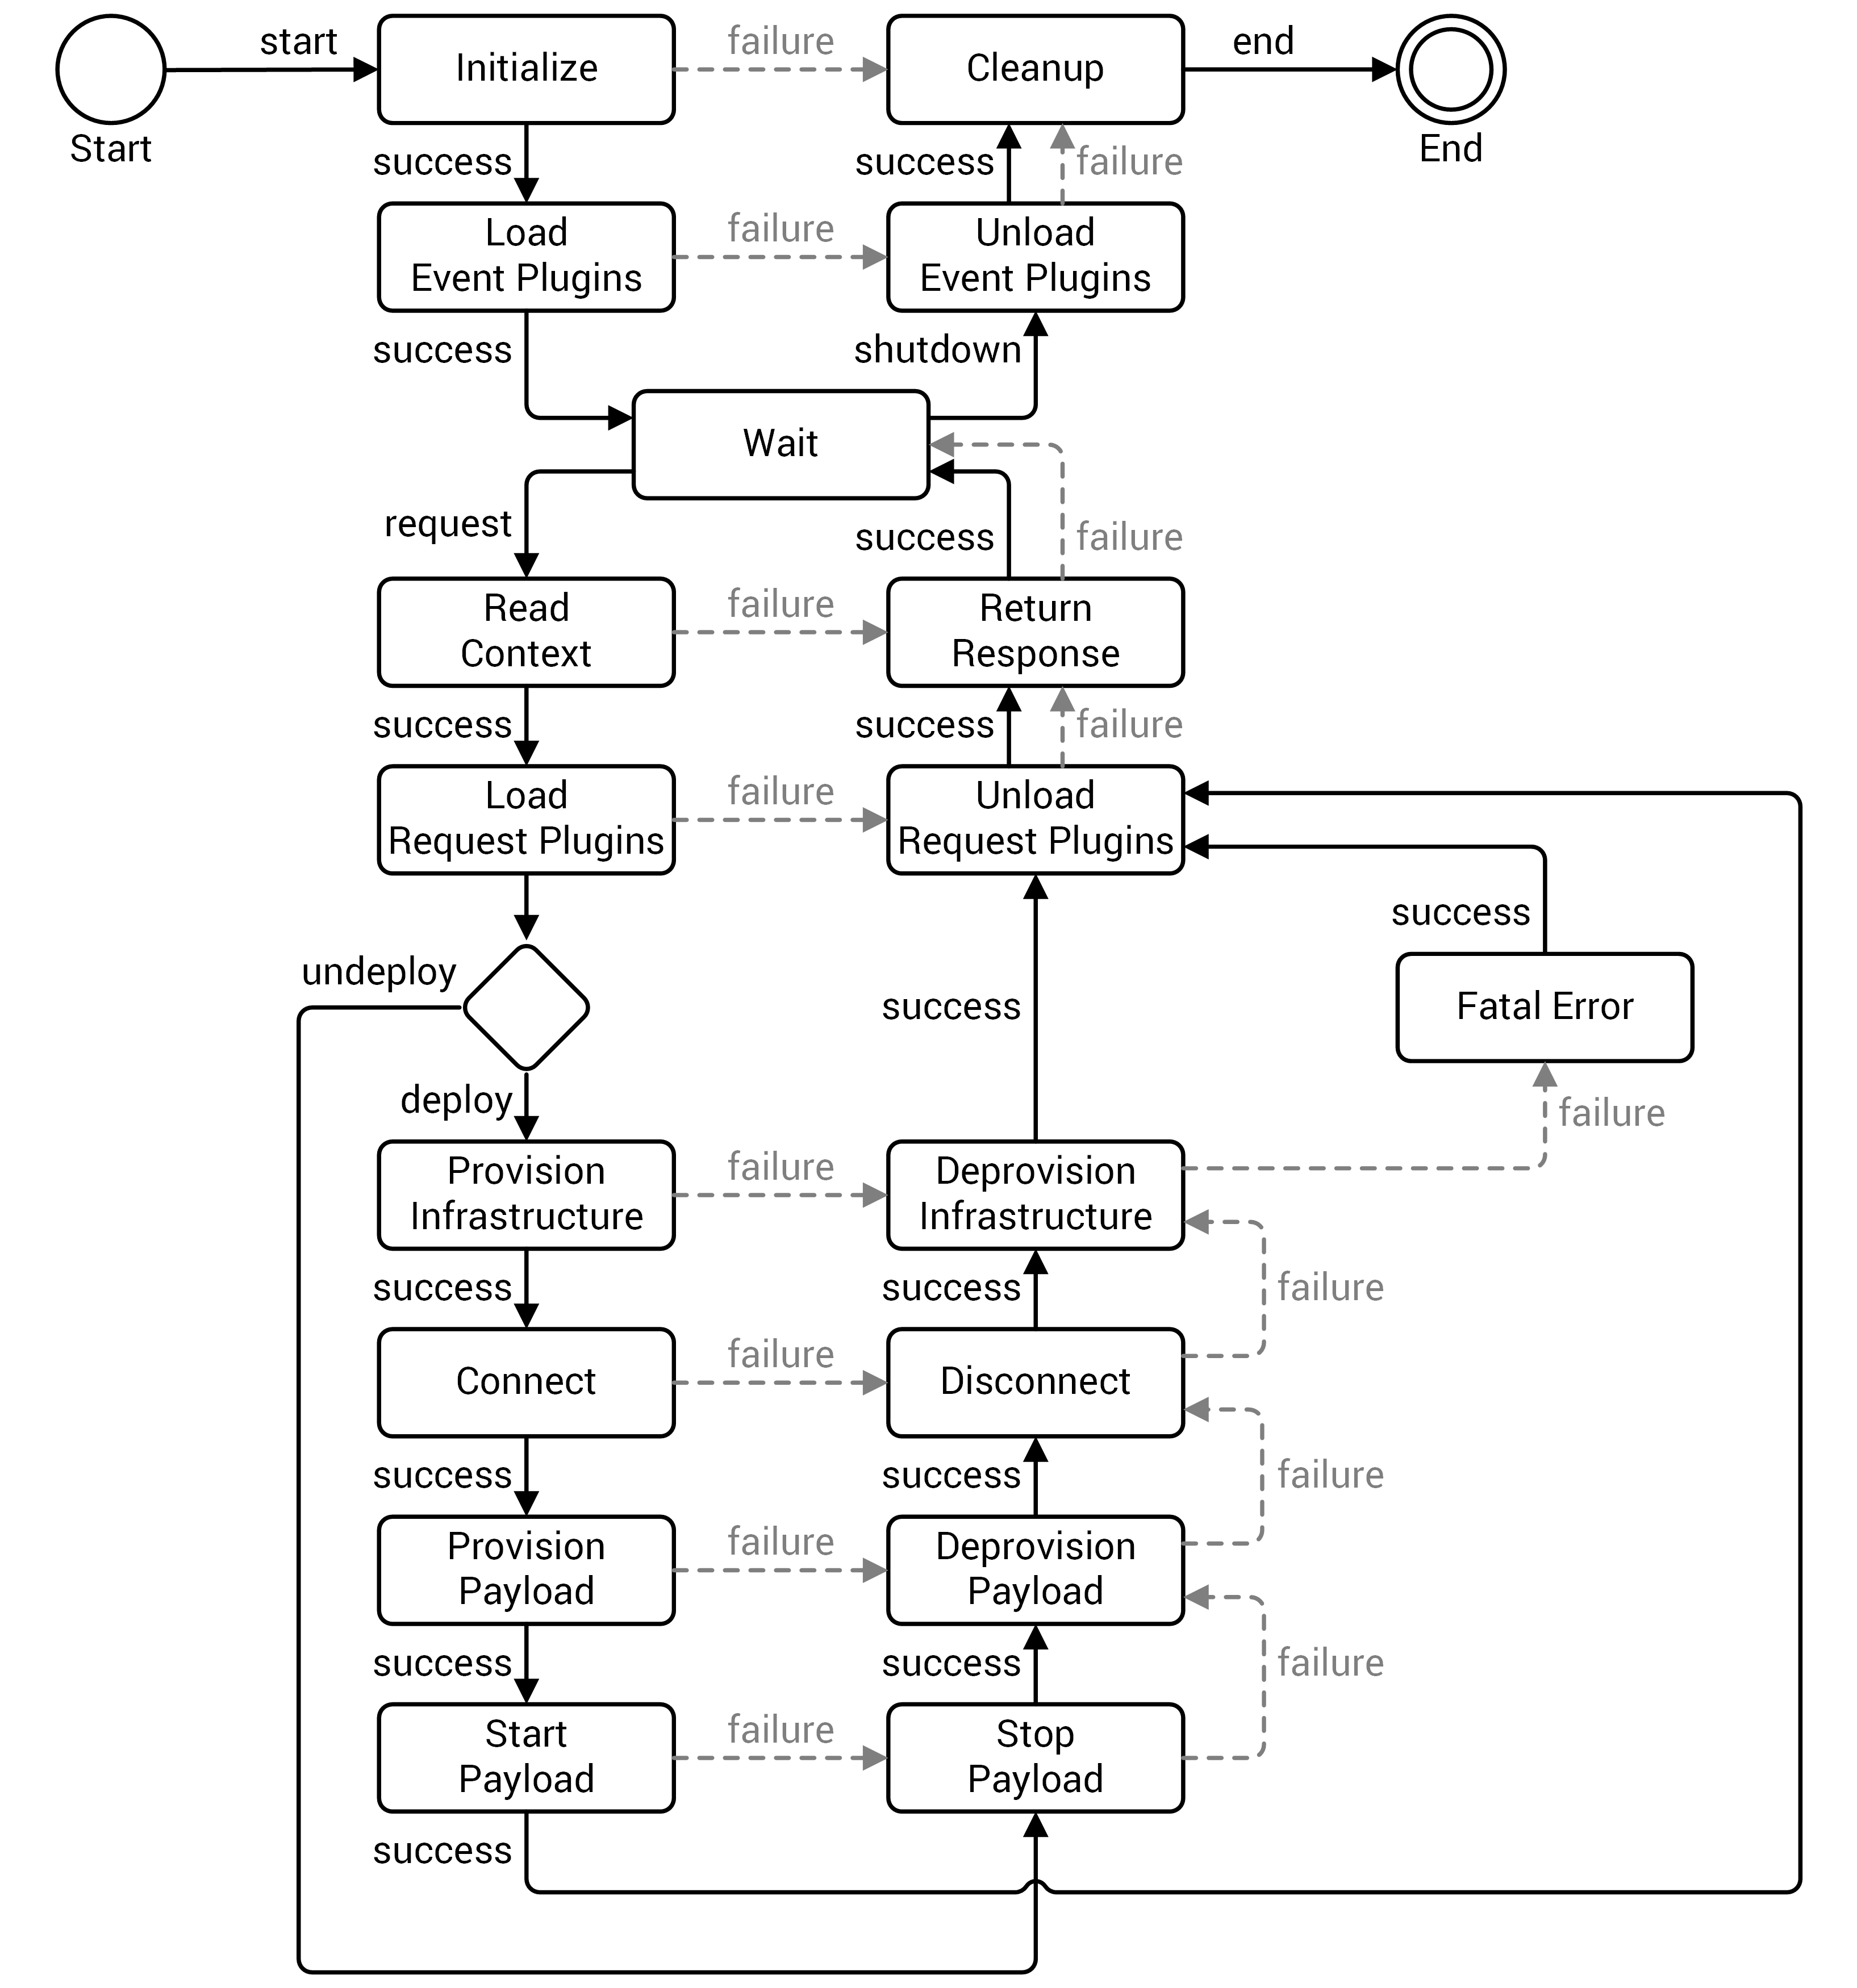
\includegraphics[resolution=600]{design/assets/flow}
	\caption{Execution flow during the bootstrapping process.}
	\label{image:flow}
\end{figure}

As \autoref{image:flow} and the description above show, this is quite a complicated process with many conditional transition.
Using traditional programming methods like if/else blocks to implement this process would lead to a rather unwieldy and complicated construct with lots of nested if/else block.
Therefore it could be advantageous to use other methods that are more fitting for this process.
Since we already describes the process as a directed graph with states and transition, it would be ideal if we could take this whole graph and use it in the bootware.
Fortunately this is possible by implementing the process using a \nom{finite state machine}{FSM}.
